%-----------------------------------------------------------------------
%\subsection{Mode and Level}
%-----------------------------------------------------------------------
%\tbc
%Baseliyos Jacob

\section{Proof of concept on the Track Utrecht Amsterdam User Stories 1 - 4}

The goal of the openETCS@ITEA2 project is to deliver at the and a proof of concept in a lab on a real ETCS Track. Since the Level 2 Utrecht - Amsterdam track was evaluated as the most approriate reference track for this concept due the maturity and representative of the track, it will be use for the mentioned simulation.\\

To start with the realisation of the concept in a iterative way in the same pattern the industry is proceeding and an regarding the "classical" state of the art of sytemanalisiys we started in this third iteration with the following Use Cases and Scenarios:\\

\subsection{Use Case and Scenario 1}
\textbf{Start of Mission - Awakening of the Train:}
This use case according to the procedure in chapter 5 will demonstrate the start of a train from a no power modus to the state that train will be ready for level and mode change according to the chapter 5.\\ 
Link on Git-Hub \url{https://github.com/openETCS/modeling/issues/66}

The following Subsystems needs to be realised for Scenario 1:\\
\begin{itemize}
\item Procedure
\item TIU Management
\item DMI Management and Controller
\item Position Report
\item Management of Radio Communication
\item Manage Track Data
\item Manage Mode and Level
\item Train Supervision
\end{itemize}

\subsection{Use Case and Scenario 2}
\textbf{Start of Mission - Start in Level 2 Mode FS:}
This use case according to the procedure in chapter 5 will demonstrate the start of a train from the awakening of the train in mode stand by to the state that train will receive a movement authority in level 2 and change into the mode full supervision to start running under real supervision according to the chapter 5.\\ 
link on Git-Hub \url{https://github.com/openETCS/modeling/issues/67}

The following Subsystems needs to be realised for Scenario 2:\\
\begin{itemize}
\item Procedure
\item TIU Management
\item DMI Management and Controller
\item Position Report
\item Management of Radio Communication
\item Manage Track Data
\item Manage Mode and Level
\item Train Supervision
\end{itemize}

\subsection{Use Case and Scenario 3}
\textbf{Brake intervention - Revocation of a Movement Authority and Overrun Permitted Speed:}
This use case according to the subset 26 chapter 3 principles will demonstrate the brake intervention that will cause by a revocation of a movement authority due to a occupied section or track an due simple overrun of a permitted speed  according to the chapter 3.\\ 
Link on Git-Hub \url{https://github.com/openETCS/modeling/issues/68}

The following Subsystems needs to be realised for Scenario 3:\\
\begin{itemize}
\item Procedure
\item TIU Management
\item DMI Management and Controller
\item Position Report
\item Management of Radio Communication
\item Manage Track Data
\item Manage Mode and Level
\item Train Supervision
\end{itemize}

\subsection{Use Case and Scenario 4}
\textbf{ETCS Onboard Unit is reading and sending track information:}
This use case according to the subset 26 chapter 3 principles will demonstrate the full completeness and checking the reading and sending of track information in interaction with the ETCS Onboard Unit and the track that will be separated in radio and balise messages. Messages and packages are defined in chapter 7 and 8 of the subset 26.\\ 
Link on Git-Hub \url{https://github.com/openETCS/modeling/issues/69}

The following Subsystems needs to be realised for Scenario 4:\\
\begin{itemize}
\item Procedure
\item TIU Management
\item DMI Management and Controller
\item Position Report
\item Management of Radio Communication
\item Manage Track Data
\item Manage Mode and Level
\item Train Supervision
\item Building of coordinate system
\end{itemize}

\section{Environment model for the use case demonstrations}

%
% nice screenshots needed!
%
%

In order to dynamically explore and demonstrate the openETCS OBU kernel software, a dynamic simulation and demonstration environmental model is being created.
During Iteration 3, this comprises the following features and functionalities:\\
•   openETCS OBU formal model \\
•   openETCS DMI formal model with Display specification model\\
•      Simplified version, not all features are implemented yet; following our use- case driven approach we are only implementing features that are essential to show the use cases selected by our "internal customer".\\
•    Environment model with \\
•  	- simplified track model (balise locations, speed profile)\\
•  	- simplified model of Movement Authority\\
•  	- interactive widgets to manipulate the simulation environment\\
\\
\\
\\


(see Figure \ref{fig:WP3-demo}.)
	
\begin{figure}
  \centering
  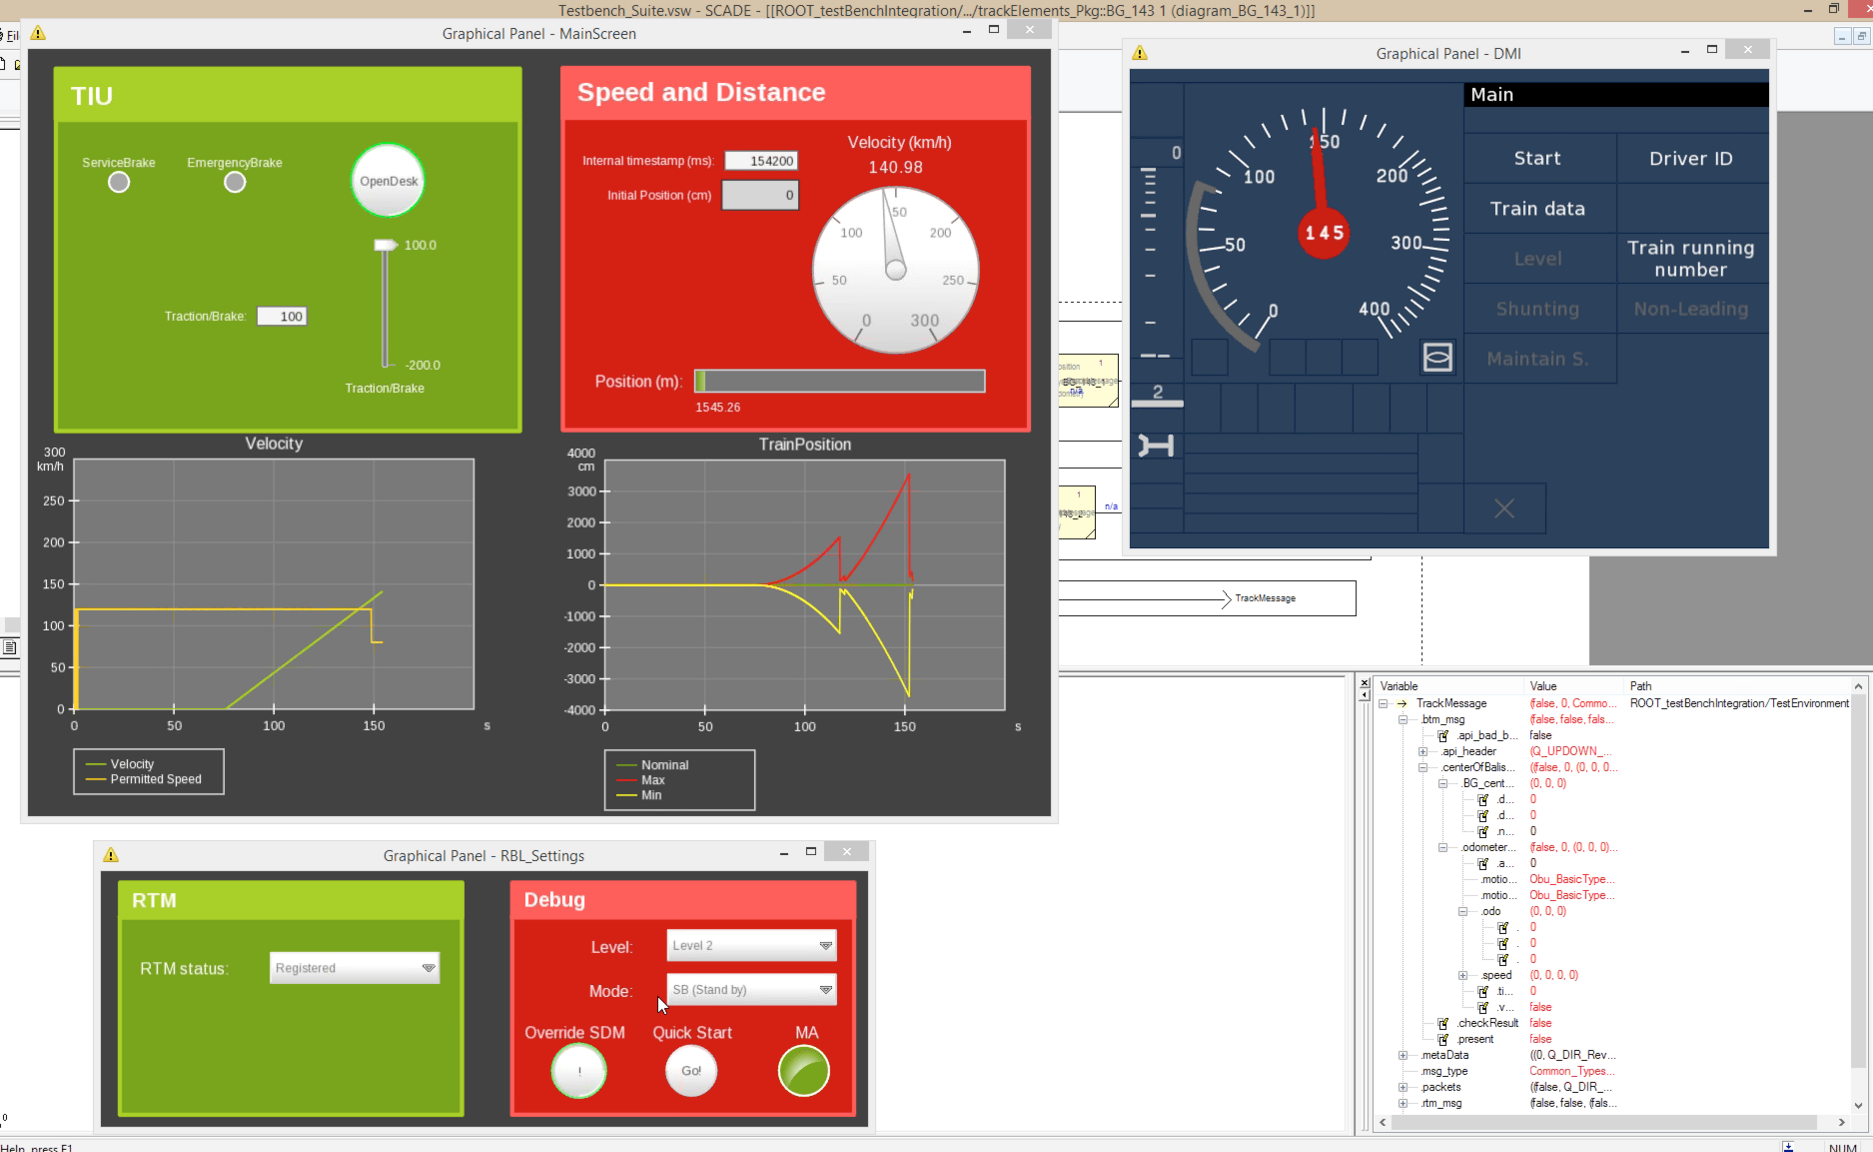
\includegraphics[width=\linewidth]{POC_environment.png}
  \caption{Environment for use case demonstration}
  \label{fig:WP3-demo}
\end{figure}




\section{Dynamic track model of the ETCS Level 2 line Amsterdam- Utrecht}

This environment model will be fourthly enhanced during the last project period, in order to:\\

•   Allow full dynamic simulation of the Utrecht- Amsterdam line\\
•   Form a basis for a (future) dynamic track simulator, which models the balise locations, balise messages and RBC messages for any given line, and which can automatically be generated from engineering datasets.\\
•   Provide a full track model for the purposes of openETCS\\
\\

(see Figure \ref{fig:track-dynamic}.)
	
\begin{figure}
  \centering
  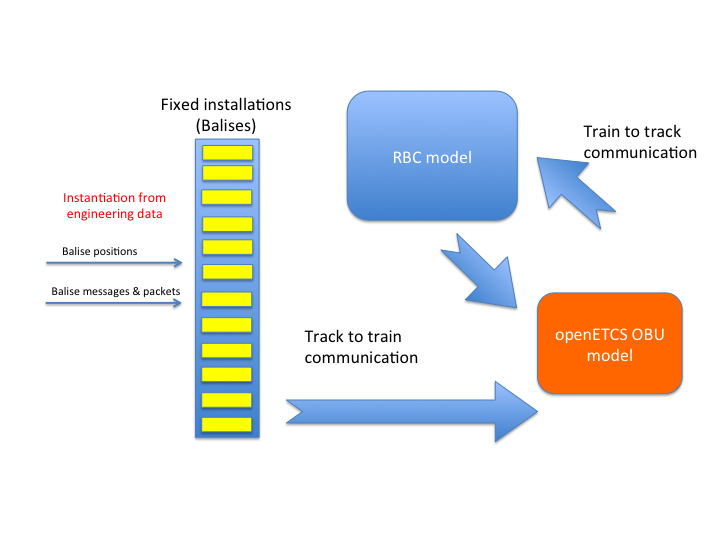
\includegraphics[width=\linewidth]{POC-track-dynamic.png}
  \caption{Schematic view of dynamic track model}
  \label{fig:track-dynamic}
\end{figure}

%
%
%
%



